\chapter{Additional results MAST}





\begin{figure}[h]
  \centering
  \subfigure[expression signatures]{
    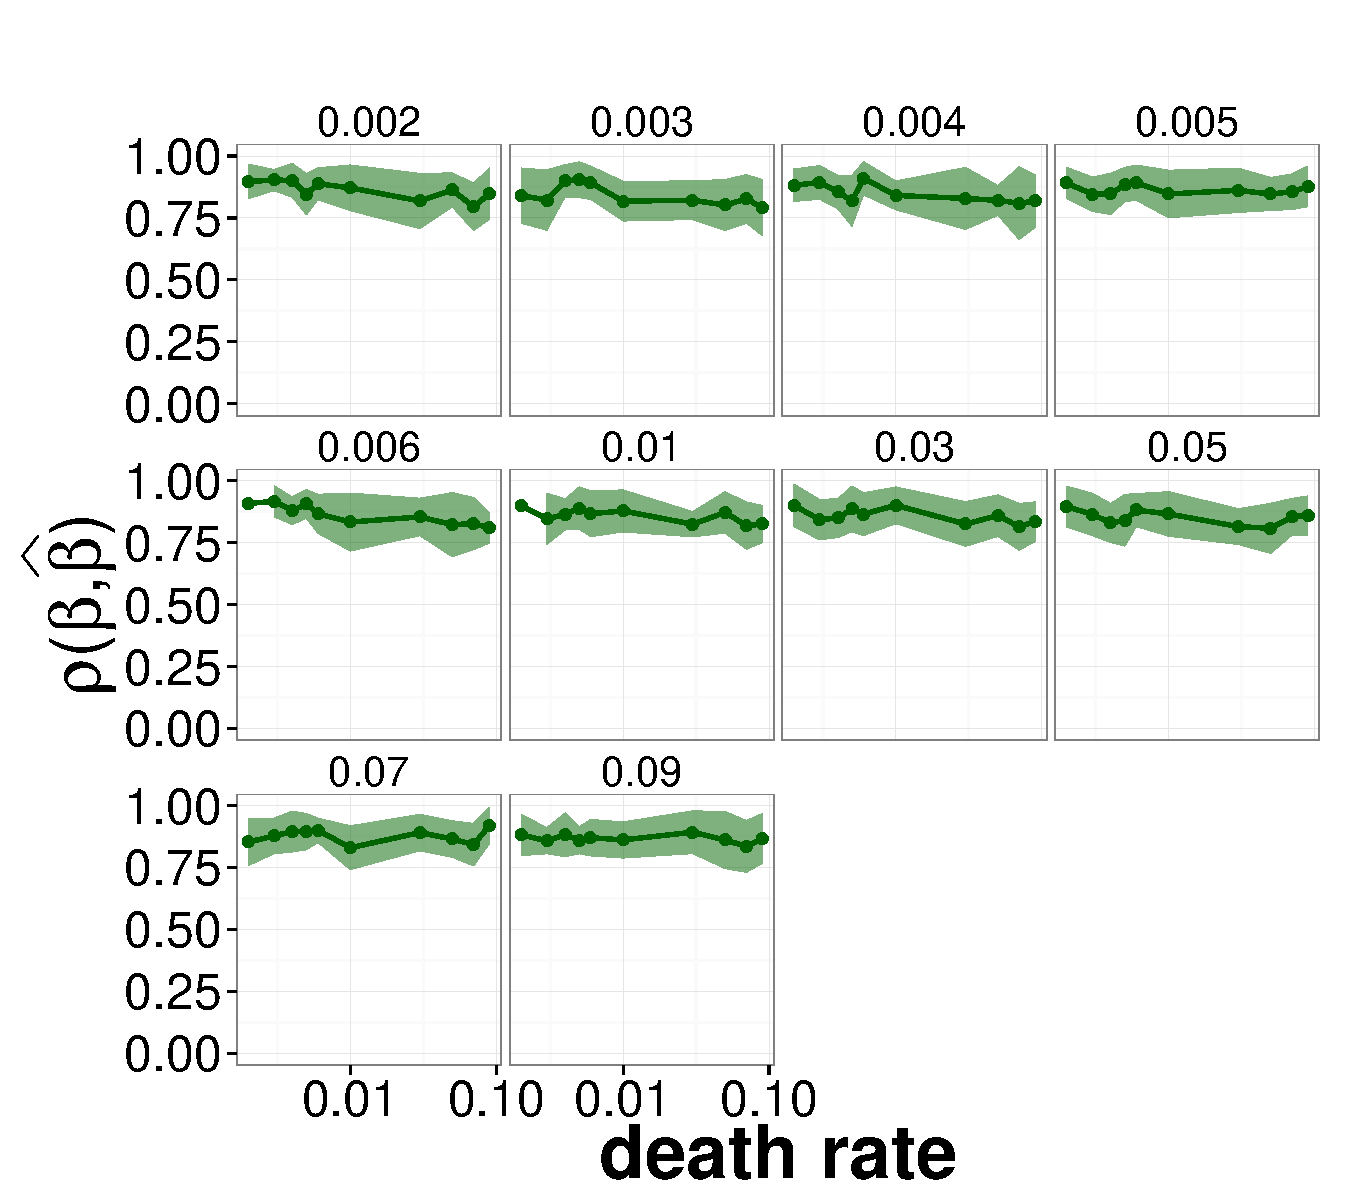
\includegraphics[width=0.7\textwidth]{pics/devide-b.pdf}
    \label{fig:devide-beta}
  }
\caption{Figure carried on below.}    
    \label{fig:dupl-all}
\end{figure}

\begin{figure}
  \ContinuedFloat
  \centering
  \subfigure[state occupation probabilities] {
    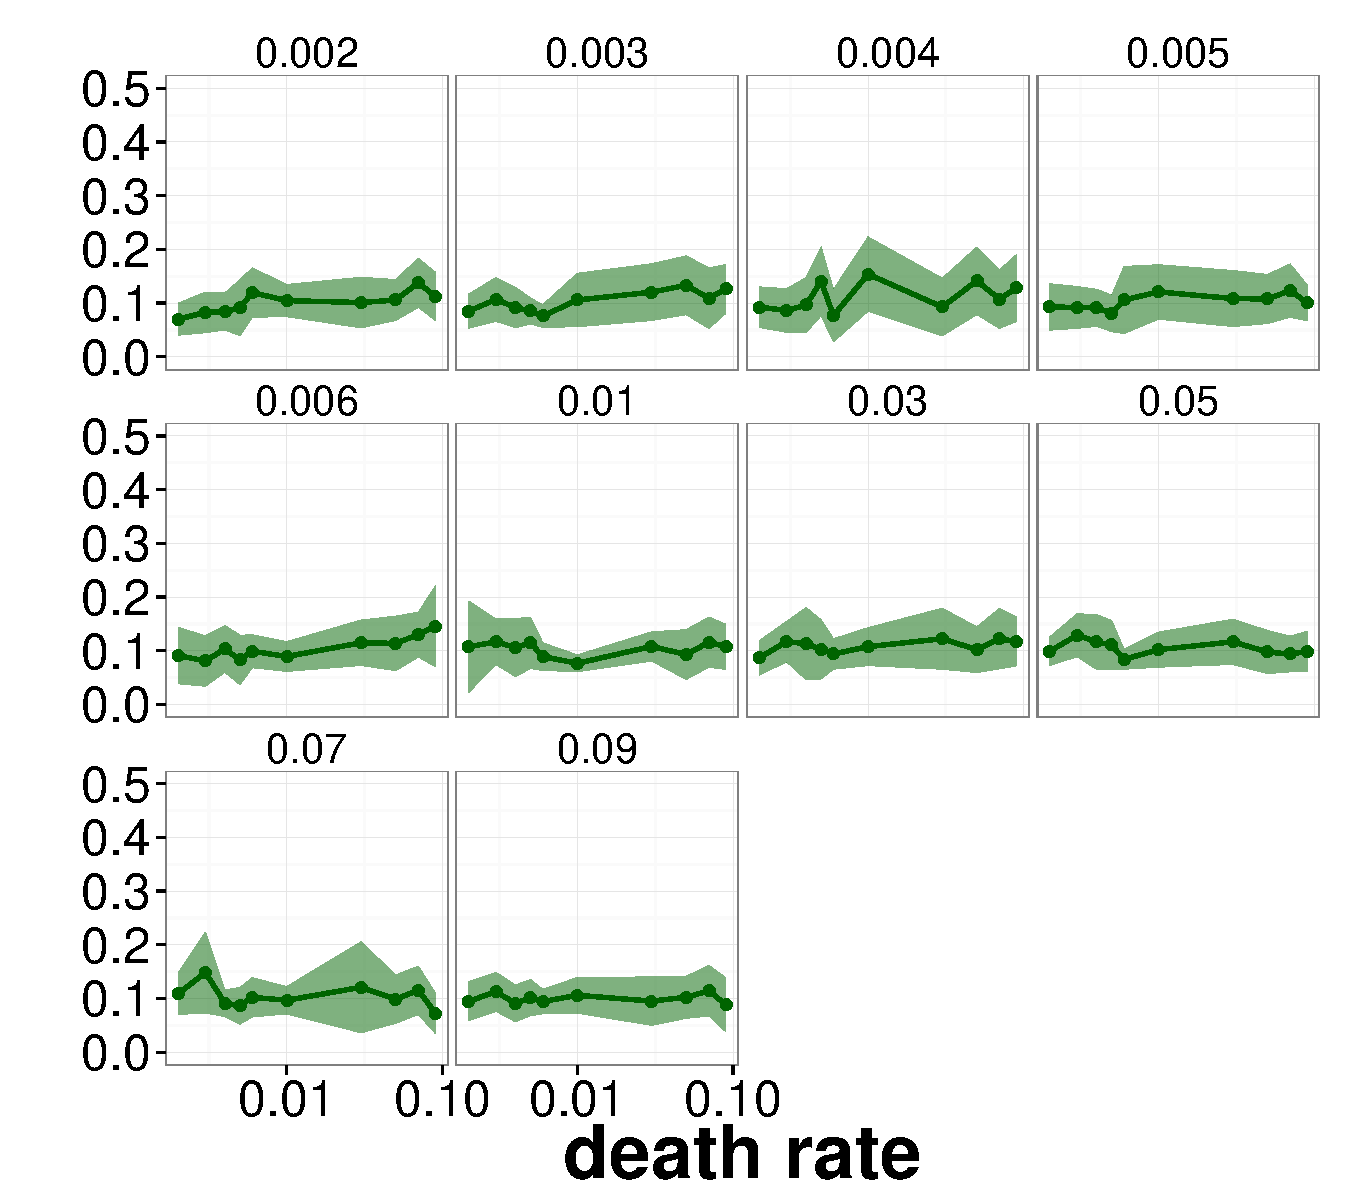
\includegraphics[width=0.7\textwidth]{pics/devide-p.pdf}
    \label{fig:devide-occ}
  }
  \subfigure[transition rate $w_{12}$] {
    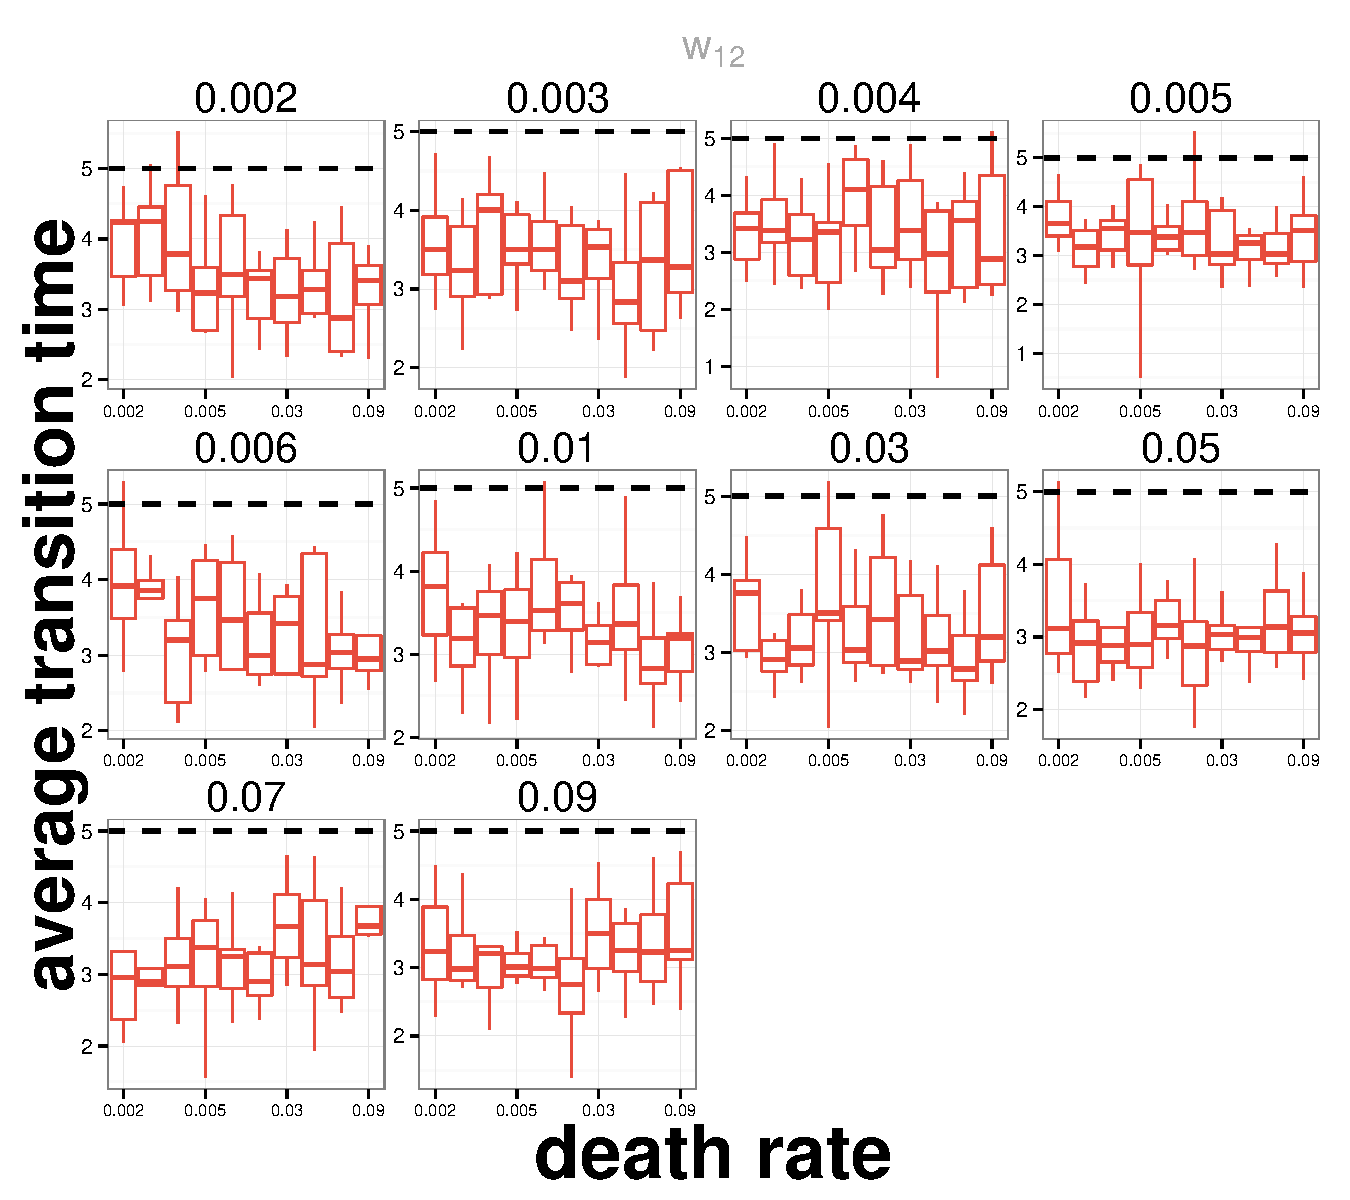
\includegraphics[width=0.7\textwidth]{pics/devide-w1.pdf}
    \label{fig:devide-w1}
  }
  \caption{Figure carried on below.}
  \label{fig:dupl-all}
\end{figure}

\clearpage
\thispagestyle{empty}
\begin{figure}
  \ContinuedFloat
  \centering
  \subfigure[transition rate $w_{23}$] {
    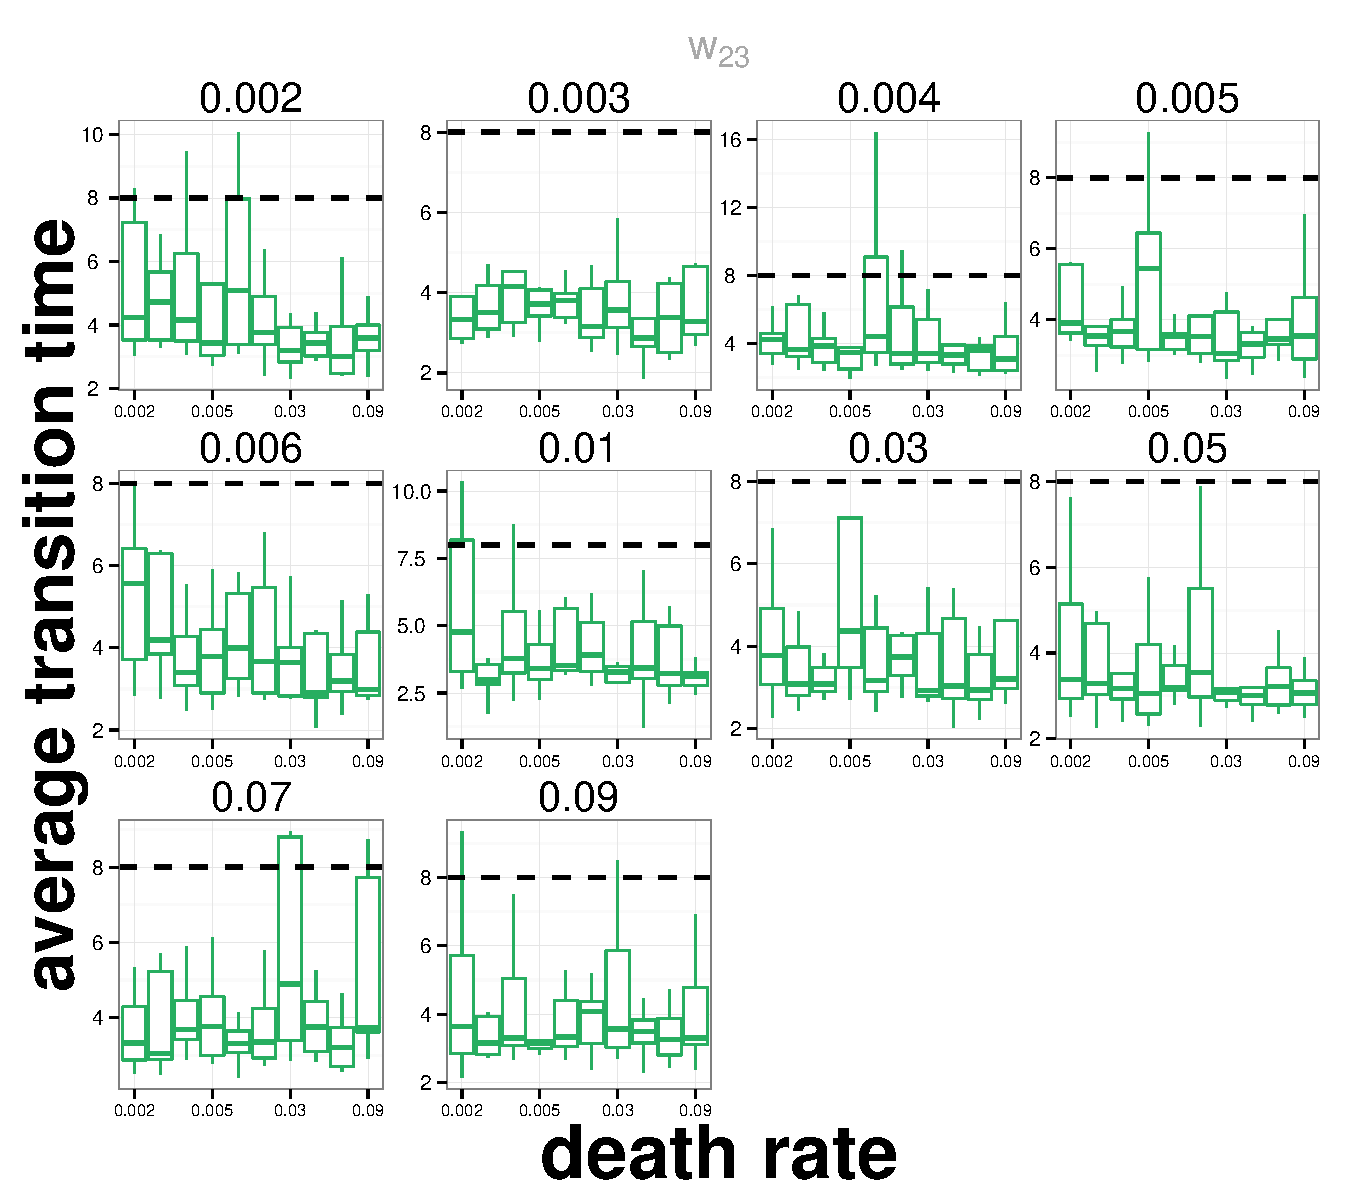
\includegraphics[width=0.7\textwidth]{pics/devide-w2.pdf}
    \label{fig:devide-w2}
  }
  \subfigure[transition rate $w_{34}$] {
    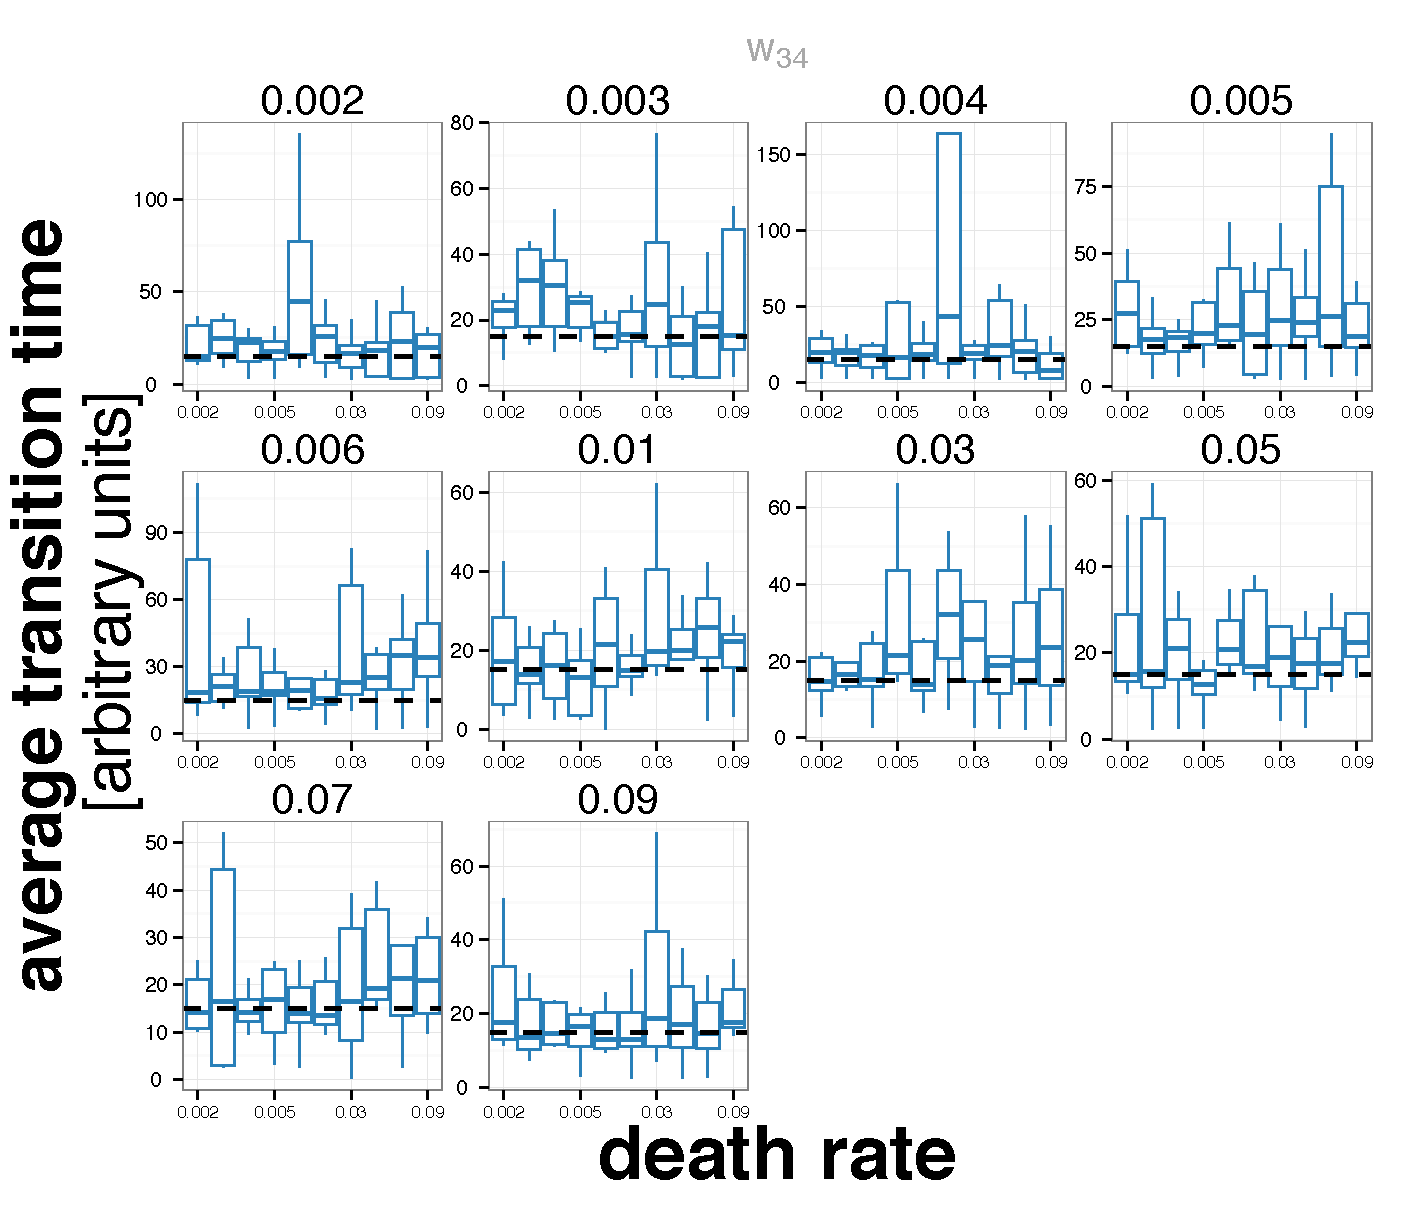
\includegraphics[width=0.7\textwidth]{pics/devide-w3.pdf}
    \label{fig:devide-w3}
  }
  \caption{Simulation study. This plots extends Figure \ref{fig:dupl-realistic} to include addition values for the doubling rate, plots are divided into panels for each cell doubling rate. Simulations are independently repeated $10$ times. \subref{fig:devide-beta} shows correlation between true and estimated $\beta_{kj}$ as a function of death rates. \subref{fig:devide-occ} shows difference between estimated occupation probabilities and true values (see Section \ref{sec:viol-model-assumpt}). In \subref{fig:devide-beta} and \subref{fig:devide-occ} show the mean as a solid line and the shaded area represents the standard deviation. \subref{fig:devide-w1} - \subref{fig:devide-w3} shows box plots for estimated transition rates with the dashed line showing true values.}
  \label{fig:dupl-all}
\end{figure}
\clearpage

\begin{figure}
  \centering
  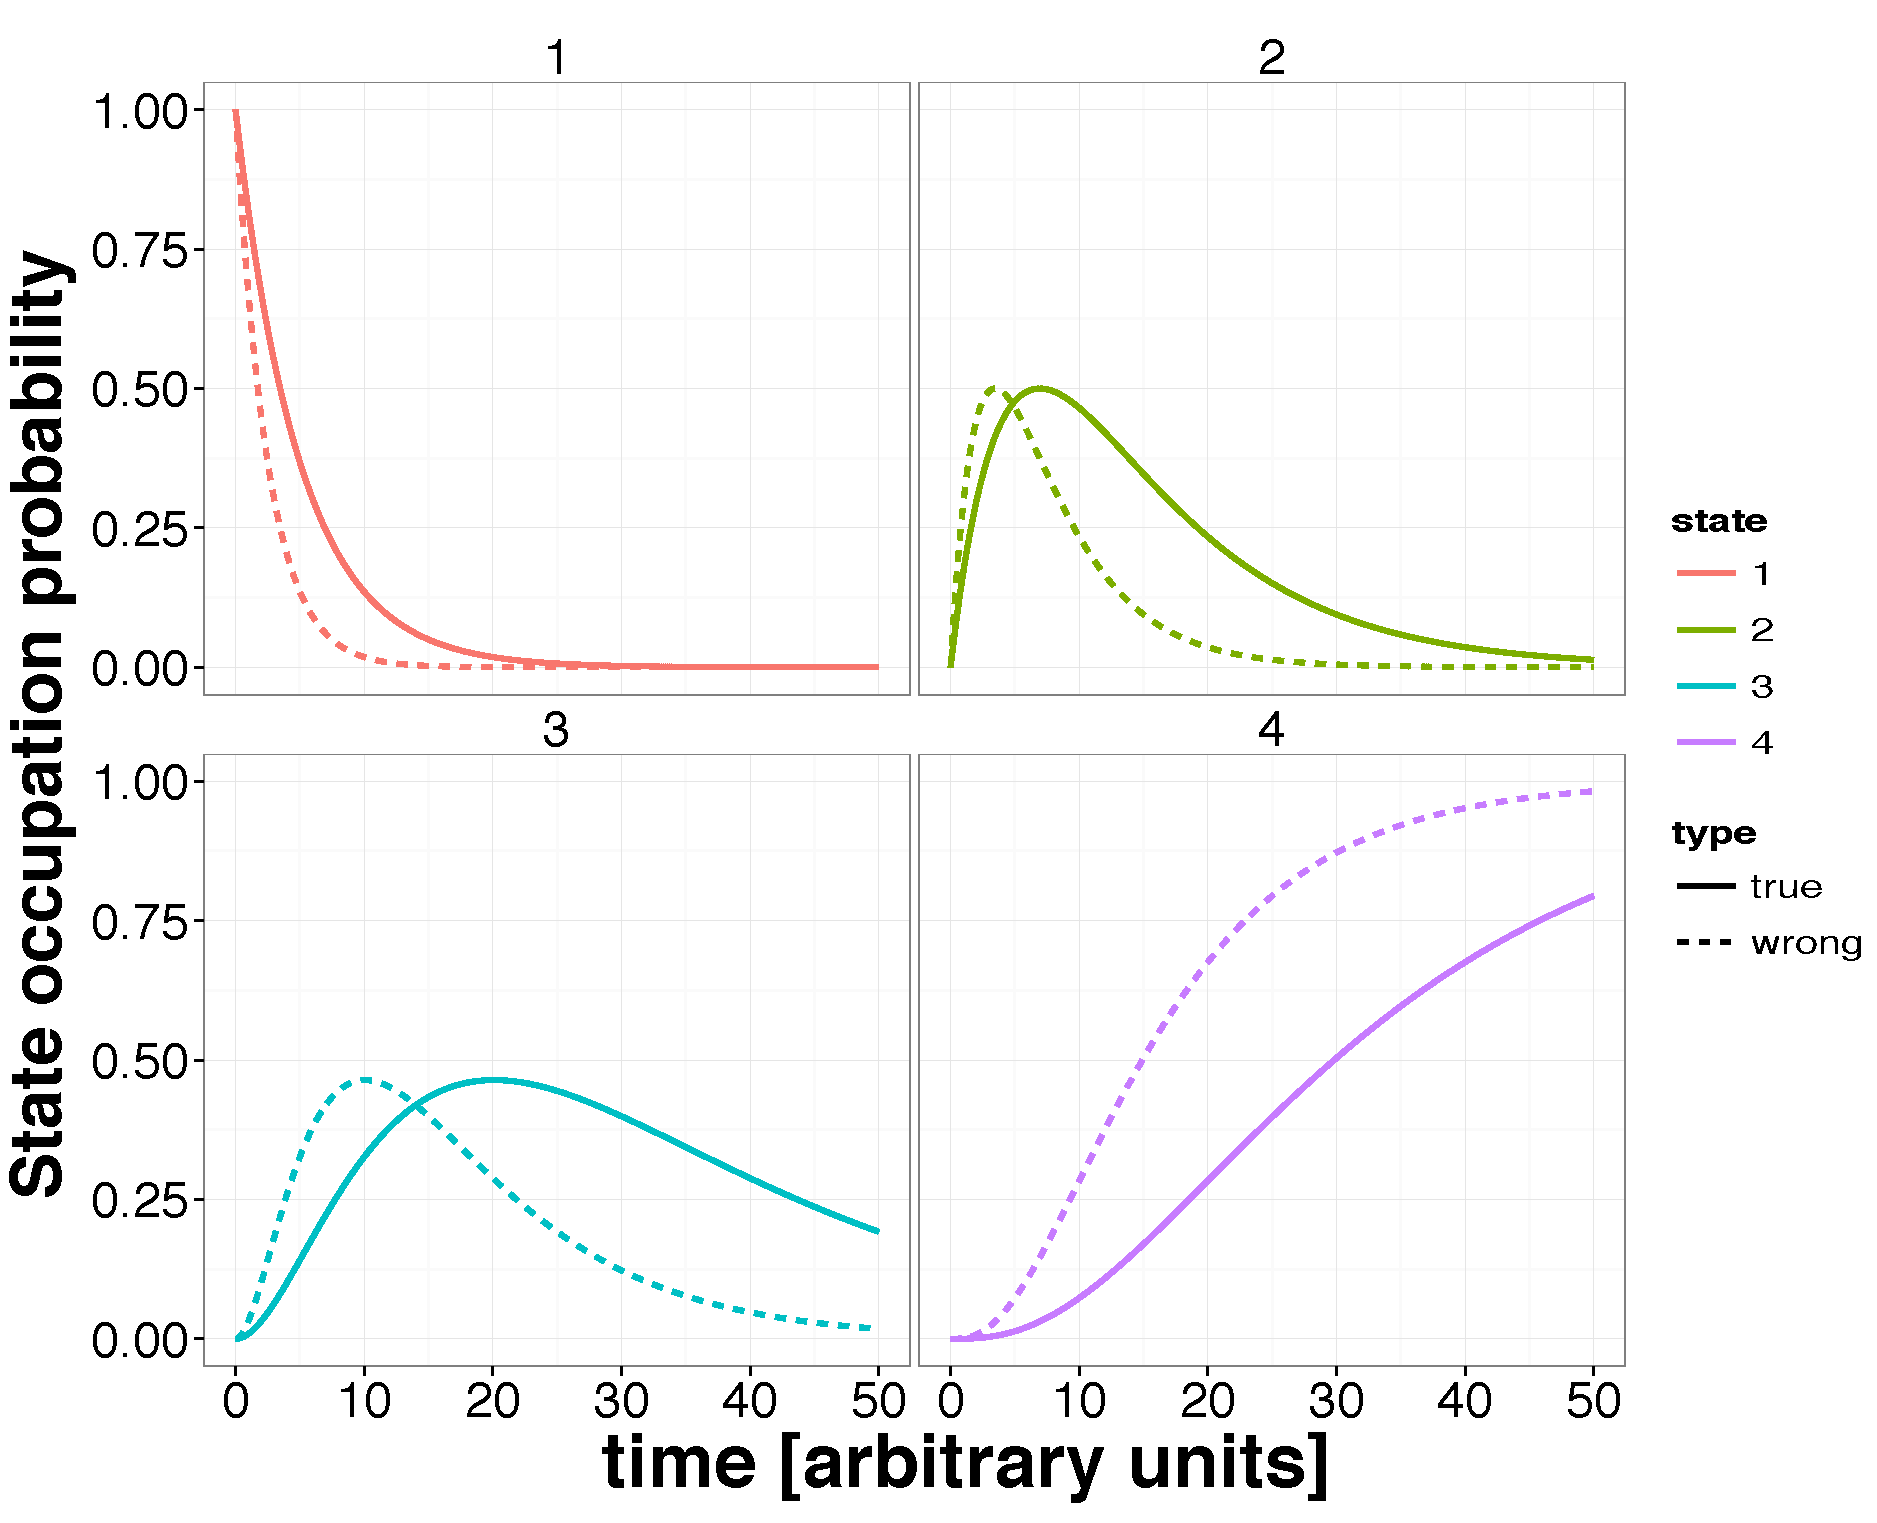
\includegraphics[width=0.9\textwidth]{pics/wrong_w.pdf}
  \caption{Simulation study. To highlight the effect of badly estimated transition rates we show state occupation probabilities for each state. The solid line shows probabilities for transition rates $[0.2, 0.1, 0.05]$ the dashed line shows occupation probabilities with transition rates $[0.4, 0.2, 0.1]$. This shows  that estimating transition rates is a more difficult problem. }
  \label{fig:wrong_w}
\end{figure}

% \caption{Simulation study. Extends Figure \ref{fig:dupl-realistic} to include more parameters for the  doubling rate. The top left panel shows correlation between true and estimated $\beta_{kj}$ as a function of death rates. The bottom left panel shows mean differences between estimated and true probabilities. In both the average over $10$ trajectories is a solid line and the shaded area is the standard deviation. The remaining panels summarise estimated Different panels show a range of doubling rates. The remaining panels show boxplots for the estimated average transition times the horizontal dashed line shows the true values used in estimation. }

% \begin{figure}
%   \centering 
%   \subfloat[][]{...figure code...}% 
%   \qquad 
%   \subfloat[][]{...figure code...} 
%   \caption{Here are the first two figures of a continued figure.}
%   \label{fig:cont}
% \end{figure}

% \begin{figure}
%   \ContinuedFloat 
%   \centering 
%   \subfloat[][]{...figure code...}% 
%   \qquad 
%   \subfloat[][]{...figure code...} 
%   \caption[]{Here are the last two figures of a continued figure.}
%   \label{fig:cont}
% \end{figure} 

%%% Local Variables:
%%% TeX-master: "warwickthesis"
%%% End:
